\documentclass[]{article}
\usepackage{lmodern}
\usepackage{amssymb,amsmath}
\usepackage{ifxetex,ifluatex}
\usepackage{fixltx2e} % provides \textsubscript
\ifnum 0\ifxetex 1\fi\ifluatex 1\fi=0 % if pdftex
  \usepackage[T1]{fontenc}
  \usepackage[utf8]{inputenc}
\else % if luatex or xelatex
  \ifxetex
    \usepackage{mathspec}
    \usepackage{xltxtra,xunicode}
  \else
    \usepackage{fontspec}
  \fi
  \defaultfontfeatures{Mapping=tex-text,Scale=MatchLowercase}
  \newcommand{\euro}{€}
\fi
% use upquote if available, for straight quotes in verbatim environments
\IfFileExists{upquote.sty}{\usepackage{upquote}}{}
% use microtype if available
\IfFileExists{microtype.sty}{%
\usepackage{microtype}
\UseMicrotypeSet[protrusion]{basicmath} % disable protrusion for tt fonts
}{}
\usepackage[margin=1in]{geometry}
\usepackage{color}
\usepackage{fancyvrb}
\newcommand{\VerbBar}{|}
\newcommand{\VERB}{\Verb[commandchars=\\\{\}]}
\DefineVerbatimEnvironment{Highlighting}{Verbatim}{commandchars=\\\{\}}
% Add ',fontsize=\small' for more characters per line
\usepackage{framed}
\definecolor{shadecolor}{RGB}{248,248,248}
\newenvironment{Shaded}{\begin{snugshade}}{\end{snugshade}}
\newcommand{\KeywordTok}[1]{\textcolor[rgb]{0.13,0.29,0.53}{\textbf{{#1}}}}
\newcommand{\DataTypeTok}[1]{\textcolor[rgb]{0.13,0.29,0.53}{{#1}}}
\newcommand{\DecValTok}[1]{\textcolor[rgb]{0.00,0.00,0.81}{{#1}}}
\newcommand{\BaseNTok}[1]{\textcolor[rgb]{0.00,0.00,0.81}{{#1}}}
\newcommand{\FloatTok}[1]{\textcolor[rgb]{0.00,0.00,0.81}{{#1}}}
\newcommand{\CharTok}[1]{\textcolor[rgb]{0.31,0.60,0.02}{{#1}}}
\newcommand{\StringTok}[1]{\textcolor[rgb]{0.31,0.60,0.02}{{#1}}}
\newcommand{\CommentTok}[1]{\textcolor[rgb]{0.56,0.35,0.01}{\textit{{#1}}}}
\newcommand{\OtherTok}[1]{\textcolor[rgb]{0.56,0.35,0.01}{{#1}}}
\newcommand{\AlertTok}[1]{\textcolor[rgb]{0.94,0.16,0.16}{{#1}}}
\newcommand{\FunctionTok}[1]{\textcolor[rgb]{0.00,0.00,0.00}{{#1}}}
\newcommand{\RegionMarkerTok}[1]{{#1}}
\newcommand{\ErrorTok}[1]{\textbf{{#1}}}
\newcommand{\NormalTok}[1]{{#1}}
\usepackage{graphicx}
\makeatletter
\def\maxwidth{\ifdim\Gin@nat@width>\linewidth\linewidth\else\Gin@nat@width\fi}
\def\maxheight{\ifdim\Gin@nat@height>\textheight\textheight\else\Gin@nat@height\fi}
\makeatother
% Scale images if necessary, so that they will not overflow the page
% margins by default, and it is still possible to overwrite the defaults
% using explicit options in \includegraphics[width, height, ...]{}
\setkeys{Gin}{width=\maxwidth,height=\maxheight,keepaspectratio}
\ifxetex
  \usepackage[setpagesize=false, % page size defined by xetex
              unicode=false, % unicode breaks when used with xetex
              xetex]{hyperref}
\else
  \usepackage[unicode=true]{hyperref}
\fi
\hypersetup{breaklinks=true,
            bookmarks=true,
            pdfauthor={Carlos Espino García},
            pdftitle={Tooth Growth Inferential Data Analysis},
            colorlinks=true,
            citecolor=blue,
            urlcolor=blue,
            linkcolor=magenta,
            pdfborder={0 0 0}}
\urlstyle{same}  % don't use monospace font for urls
\setlength{\parindent}{0pt}
\setlength{\parskip}{6pt plus 2pt minus 1pt}
\setlength{\emergencystretch}{3em}  % prevent overfull lines
\setcounter{secnumdepth}{5}

%%% Use protect on footnotes to avoid problems with footnotes in titles
\let\rmarkdownfootnote\footnote%
\def\footnote{\protect\rmarkdownfootnote}

%%% Change title format to be more compact
\usepackage{titling}

% Create subtitle command for use in maketitle
\newcommand{\subtitle}[1]{
  \posttitle{
    \begin{center}\large#1\end{center}
    }
}

\setlength{\droptitle}{-2em}
  \title{Tooth Growth Inferential Data Analysis}
  \pretitle{\vspace{\droptitle}\centering\huge}
  \posttitle{\par}
  \author{Carlos Espino García}
  \preauthor{\centering\large\emph}
  \postauthor{\par}
  \predate{\centering\large\emph}
  \postdate{\par}
  \date{July 22, 2015}



\begin{document}

\maketitle


\section{Overview}

This project analyzes the influence of supplement type and dose level on
tooth growth of guinea pigs. To do this, ee consider two types of
supplement (Vitamin C and Orange Juice) and three levels of dose (0.5mg,
1mg and 2mg) and we examine the difference of tooth length among
different groups by hypothesis testing.

\section{Dataset Description}

Each observation of the corresponds to the measure of length of
odontoblasts in each of 10 guinea pigs at each of three dose levels of
Vitamin C (0.5, 1, and 2 mg) with each of two delivery methods (orange
juice or ascorbic acid).

\begin{enumerate}
\def\labelenumi{\arabic{enumi}.}
\itemsep1pt\parskip0pt\parsep0pt
\item
  \textbf{len}: is the length of odontoblasts (teeth) in each of 10
  guinea pigs.
\item
  \textbf{supp}: corresponds to the two delivery methods (orange juice
  or ascorbic acid).
\item
  \textbf{dose}: corresponds the levels of Vitamin C (0.5, 1, and 2 mg)
\end{enumerate}

\section{Exploratory Analysis}

The table shows the mean length of the t

\begin{table}[ht]
\centering
\begin{tabular}{llr}
  \hline
supp & dose & mean(len) \\ 
  \hline
OJ & 0.5 & 13.23 \\ 
  OJ & 1 & 22.70 \\ 
  OJ & 2 & 26.06 \\ 
  VC & 0.5 & 7.98 \\ 
  VC & 1 & 16.77 \\ 
  VC & 2 & 26.14 \\ 
   \hline
\end{tabular}
\end{table}

\begin{figure}

{\centering 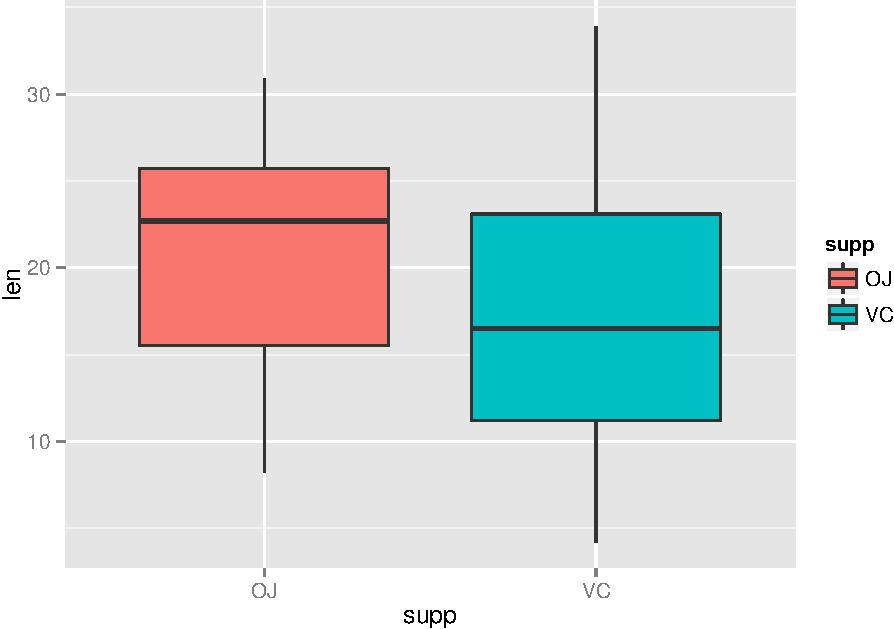
\includegraphics[width=.7\textwidth]{Tooth_Growth_Inferential_Data_Analysis_files/figure-latex/bp_by_supp-1} 

}

\caption{Boxplot by supplement type}\label{fig:bp_by_supp}
\end{figure}

\begin{figure}

{\centering 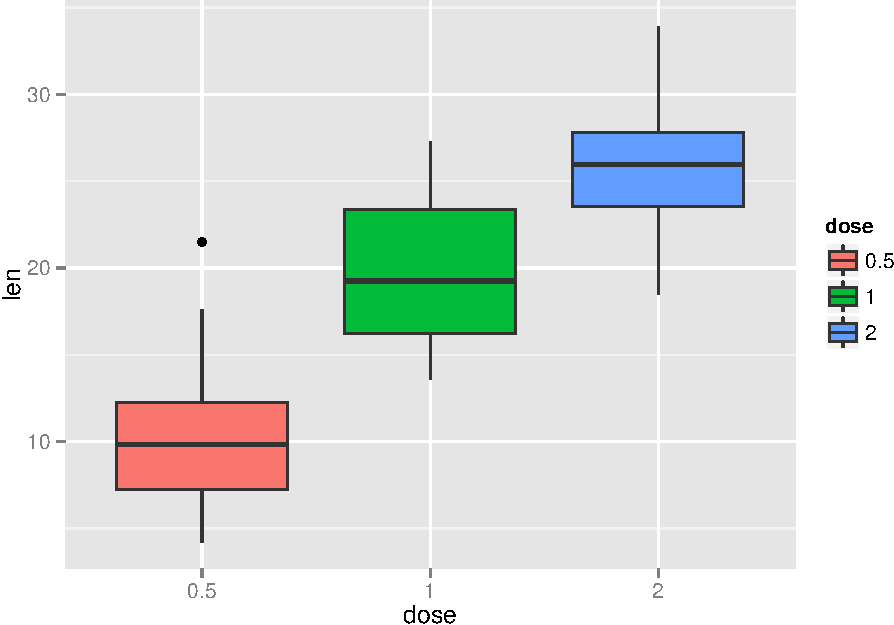
\includegraphics[width=.7\textwidth]{Tooth_Growth_Inferential_Data_Analysis_files/figure-latex/bp_by_dose-1} 

}

\caption{Boxplot by dose}\label{fig:bp_by_dose}
\end{figure}

\begin{figure}

{\centering 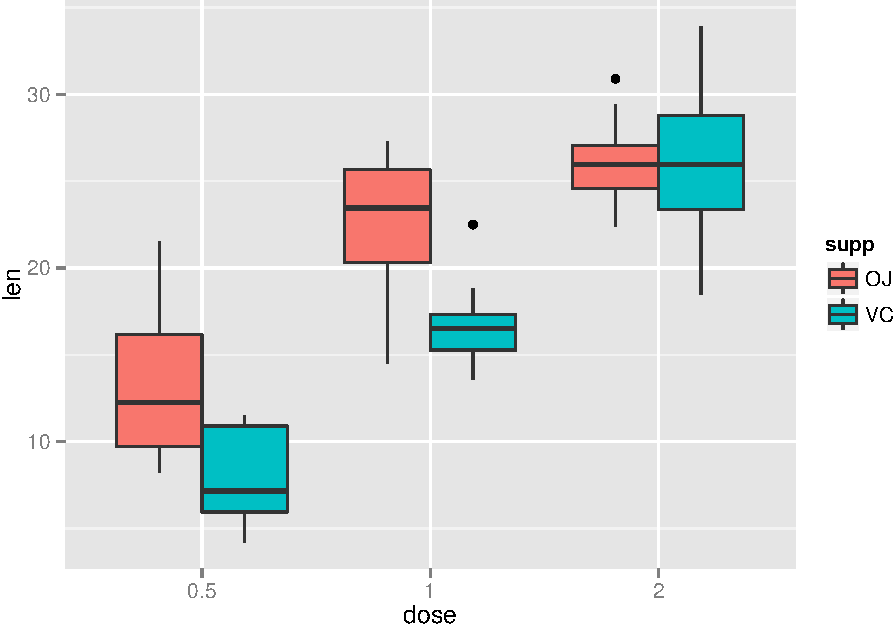
\includegraphics[width=.7\textwidth]{Tooth_Growth_Inferential_Data_Analysis_files/figure-latex/bp_by_dose_and_supp-1} 

}

\caption{Boxplot by dose}\label{fig:bp_by_dose_and_supp}
\end{figure}

\begin{Shaded}
\begin{Highlighting}[]
\KeywordTok{ggplot}\NormalTok{(ToothGrowth) +}\StringTok{ }\KeywordTok{geom_boxplot}\NormalTok{(}\KeywordTok{aes}\NormalTok{(}\DataTypeTok{x =} \NormalTok{supp, }\DataTypeTok{y =} \NormalTok{len, }\DataTypeTok{fill =}\NormalTok{dose)) }
\end{Highlighting}
\end{Shaded}

\begin{figure}

{\centering 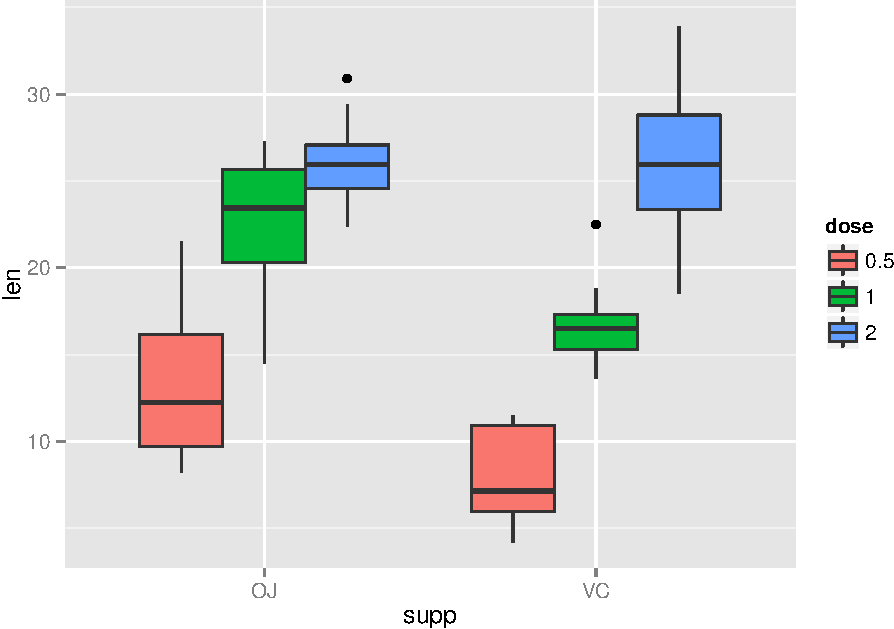
\includegraphics[width=.7\textwidth]{Tooth_Growth_Inferential_Data_Analysis_files/figure-latex/bp_by_supp_and_dose-1} 

}

\caption{Boxplot by dose}\label{fig:bp_by_supp_and_dose}
\end{figure}

You can also embed plots, for example:

\begin{figure}[htbp]
\centering
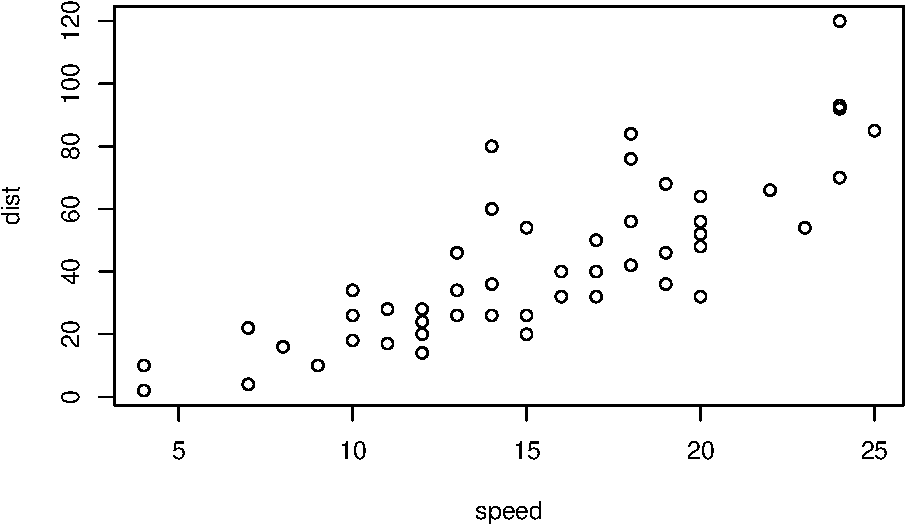
\includegraphics{Tooth_Growth_Inferential_Data_Analysis_files/figure-latex/unnamed-chunk-2-1.pdf}
\caption{}
\end{figure}

Note that the \texttt{echo = FALSE} parameter was added to the code
chunk to prevent printing of the R code that generated the plot.

\end{document}
